\documentclass[a4paper, 12pt]{article}

\usepackage[a4paper, inner=2cm, outer=2cm, top=2cm, bottom=2cm]{geometry}
\usepackage[utf8]{inputenc}
\usepackage[IL2]{fontenc}
\usepackage[czech]{babel}
\usepackage{graphicx}
\usepackage{xcolor}
\usepackage{amsmath}
\usepackage{amssymb}
\usepackage{caption}
\usepackage{algorithm}
\usepackage{algpseudocode}
\usepackage{marginnote}
\usepackage[numbers]{natbib}
\usepackage{tocloft}
\usepackage{hyperref}
\usepackage{multirow}

\renewcommand{\thealgorithm}{\arabic{section}.\arabic{algorithm}}
\renewcommand{\bibsection}{\section*{Odkazy}}
\renewcommand{\cftsecleader}{\cftdotfill{\cftdotsep}}

\bibpunct{\textcolor{blue}{[}}{\textcolor{blue}{]}}{,}{n}{}{;}
\graphicspath{{./img/}}
\hypersetup{
    colorlinks=true,
    citecolor=blue,
    linkcolor=black,
    urlcolor=blue
}

\begin{document}
\begin{titlepage}
    \begin{titlepage}
	\begin{center}
		\vspace*{1cm}
		
\includegraphics[width=8cm]{ZCU_logo}
		\vspace{3cm}

		\Large{Západočeská Univerzita v Plzni}
		\vspace{0.5cm}

		\large{Fakulta Aplikovaných Věd}
		\vspace{0.5cm}

		\large{Informatika}
		\vspace{1cm}

   		\Huge{\textbf{Semestrální práce}}
   		\vspace{0.8cm}

		\LARGE{Celočíselná kalkulačka s neomezenou přesností}
	\end{center}
	
  	\vfill

  	\LARGE{Hynek Moudrý}
	\hfill
	\Large{2022/2023}

	\Large{KIV/PC}
\end{titlepage}
\end{titlepage}

\setcounter{page}{1}
\tableofcontents
\newpage

\section{Zadání}
Naprogramujte v jazyce ANSI C konzolovou aplikaci, která bude fungovat jako jednoduchý interpret aritmetických výrazů zapsaných v infixové formě. Vstupem programu bude kromě řídících příkazů i seznam aritmetických výrazů obsahující celočíselné operandy ($\mathbb{Z}$) s neomezenou velikostí, zapsané ve dvojkové, desítkové či šestnáctkové číselné soustavě. Pro kódování operandů zapsaných ve dvojkové či šestnáctkové soustavě bude použit výhradně dvojkový doplňkový kód. Výstupem je pak odpovídající seznam výsledků vyhodnocení každého výrazu.

Program bude spouštěn příkazem \verb|calc.exe [<vstupní-soubor>]|. \\Symbol \verb|<vstupní-soubor>| zastupuje nepovinný parametr – název vstupního souboru se seznamem aritmetických výrazů. Není-li symbol \verb|<vstupní-soubor>| uveden, program bude fungovat v interaktivním módu, kdy se příkazy budou provádět přímo zadáním z konzole do interpretu.

\subsection{Specifikace vyhodnocovaných výrazů}\label{subsection:expressions}
Výrazem může být pouze příkaz interpretu, nebo aritmetický výraz v infixové formě. Interpret
je case-insensitive (tj.~nerozlišuje velká a malá písmena). 
Minimální množina podporovaných příkazů: 
\begin{itemize}
    \item \verb|quit| \dots Ukončí interpret s návratovou hodnotou \verb|EXIT_SUCCESS|.
    \item \verb|bin| \dots Výsledky výrazů budou vypisovány ve dvojkové soustavě (prefix \verb|0b|).
    \item \verb|dec| \dots Výsledky výrazů budou vypisovány v desítkové soustavě (výchozí).
    \item \verb|hex| \dots Výsledky výrazů budou vypisovány v šestnáctkové soustavě (prefix \verb|0x|).
    \item \verb|out| \dots Vypíše aktuálně vybranou číselnou soustavu (\verb|bin|, \verb|dec| nebo \verb|hex|).
\end{itemize}
\begin{table}[h]
    \caption{Minimální množina podporovaných funkcí a operátorů.}\label{tab:function}
    \begin{tabular}{clcll}
    \hline
    \textbf{Operátor}  & \textbf{Operace}              & \textbf{Precedence} & \textbf{Arita} & \textbf{Asociativita} \\ \hline
    !                  & Faktoriál                     & 4                   & unární         & levá                  \\
    \textasciicircum{} & Umocnění                      & 4                   & binární        & pravá                 \\
    -                  & Číslo opačné                  & 3                   & unární         & pravá                 \\
    *                  & Násobení                      & 3                   & binární        &                       \\
    /                  & Celočíselné dělení            & 3                   & binární        & levá                  \\
    \%                 & Zbytek po celočíselném dělení & 2                   & binární        & levá                  \\
    +                  & Součet                        & 1                   & binární        &                       \\
    -                  & Rozdíl                        & 1                   & binární        & levá                  \\
    (                  & Levá závorka                  & 0                   &                &                       \\ 
    )                  & Pravá závorka                 & 0                   &                &                       \\ \hline
    \end{tabular}
\end{table}
Celočíselné operandy mohou být ve zpracovávaných aritmetických výrazech zadány pomocí
\begin{itemize}
    \item dvojkové soustavy (prefix \verb|0b|),
    \item desítkové soustavy (bez prefixu),
    \item nebo šestnáctkové soustavy (prefix \verb|0x|). 
\end{itemize}
Pro kódování operandů bude použit výhradně dvojkový doplňkový kód, kde obecně platí:
\begin{equation}\label{eq:twos_complement}
\begin{aligned}
    \verb|3|=\verb|0b000|\dots\verb|00011|=\mathbin{\color{red}{\verb|0b011|}}&\mathbin{\color{red}{\neq}}\mathbin{\color{red}{\verb|0b11|}}=\verb|0b111|\dots\verb|11111|=\verb|-1| \\
    \verb|11|=\verb|0b0001011|=\verb|0x0000b|=\mathbin{\color{red}{\verb|0x0b|}}&\mathbin{\color{red}{\neq}}\mathbin{\color{red}{\verb|0xb|}}=\verb|0xffffb|=\verb|0b1011|=\verb|-5|
\end{aligned}
\end{equation}

\subsection{Specifikace výstupu programu}\label{subsection:output}
Program bude vždy vypisovat výsledek právě zadaného aritmetického výrazu či příkazu interpretu. Při načtení seznamu příkazů ze souboru musí výstup odpovídat přesně výstupu spuštění programu bez parametru (interaktivní režim).

Při výpisu výsledků pomocí jejich binární či hexadecimální reprezentace je, stejně jako u vstupu, použit dvojkový doplňkový kód. Vypsán bude vždy minimální potřebný počet binárních či hexadecimálních cifer – zvýrazněná část nerovnosti~(\ref{eq:twos_complement}). 

V případě chybného zadání příkazu či aritmetického výrazu vypíše interpret chybu dle tabulky
1 v úplném zadání~\cite{bib:zadani} a pokračuje ve zpracování dalšího výrazu. 

\section{Analýza úlohy}
\subsection{Reprezentace čísel}
Důležitým problémem k vyřešení je způsob uložení neomezeně přesných celých čísel v paměti. Nejprve je nutné si uvědomit, že neomezeně velká čísla není prakticky možné v počítači ukládat. Pro naše účely se tedy omezíme na `extrémně velká' čísla, jejichž maximální, resp.~minimální velikost bude diskutována dále v sekci~\ref{subsection:mpt}. V jazyce C sám o sobě neexistuje datový typ, který by taková čísla dokázal ukládat (\verb|long long| má nejvyšší přesnost a ani zdaleka nám nevystačí) a je tedy nutné vymyslet strukturu schopnou tato čísla reprezentovat, nejlépe s co nejmenší paměťovou zátěží. 

Čísla bychom mohli reprezentovat např.~polem jednobytových znaků '1' nebo '0', jednalo by se ale o velice neefektivní techniku, jejíž použití je v úplném zadání~\cite{bib:zadani} silně nedoporučeno. Mnohem lepší alternativa je použití bitového pole~\cite{bib:bit_array}. U obyčeného pole bychom ale v paměti alokovali statickou velikost, tím pádem by pole mohlo být buď zbytečně velké nebo moc malé. Namísto staticky alokovaného pole tedy použijeme pole dynamicky realokované (dále \textit{vektor}), což nám umožní alokovat paměť nejen dostatečně velkou, ale i minimální potřebnou, pro reprezentaci čísla.

\subsection{Matematické operace}\label{subsection:operace}
Nejdůležitější operací je sčítání, která je nutným základem pro další operace. Lze se inspirovat skutečným způsobem sčítání ve výpočetní technice, které se hardwarově řeší pomocí polovičních a úplných sčítaček, jenž lze jednoduše implementovat i softwarově pomocí odpovídajících logických operací. Museli bychom ale ke každému bitu přistupovat jednotlivě, což by mohlo být lehce zdlouhavé. Efektivnější by bylo využití aritmeticko-logické jednotky, aby tyto operace udělala za nás a sčítání tedy dělala byte po bytu s tím, že si pouze ohlídáme příznakový bit \verb|CARRY| mezi byty. 

K výpočtu opačných čísel se nabízí dvojkový doplněk, tedy znegování všech bitů a přičtení jedničky. Tuto operaci pak lze jednoduše využít ve spojení se sčítáním pro zhotovení operace rozdílu.

Násobení čísel $n\cdot{} m$ můžeme implementovat naivně ($n$-krát sečteme $m$, nebo naopak), pro velká čísla by ale takové řešení trvalo příliš dlouho. Využijeme místo toho techniku násobení, která se vyučuje na základních školách při násobení dvou dekadických čísel. Tento proces je v binární soustavě ještě jednodušší než v dekadické.
\newpage

Operaci celočíselného dělení lze také implementovat naivně (od dělence odečítáme dělitel dokud můžeme), znovu by se ale jednalo o nevhodné řešení, které má alternativu opět v technice dělení ze základních škol.

Řešení pro výpočet zbytku po celočíselném dělení je zmíněn v zadání~\cite{bib:zadani}, implementujeme ho tedy stejně jako je implementován překladačemi jazyka ANSI~C:\@
\begin{equation}
    a\%m=a-m\left\lfloor\frac{a}{m}\right\rfloor
\end{equation}

Umocnění základu exponentem je další naivně implementovatelnou operací, pro vylepšení zde ale žádnou techniku ze základní školy nevyužijeme. Pro efektivnější výpočet mocniny v binární soustavě existuje velice jednoduchý a rychlý algoritmus~\cite{bib:power} popsaný dále v sekci~\ref{subsection:mpt_operace}.

Poslední operací je faktoriál, který je neproblematičtější a pravděpodobně neexistuje jiné řešení, než postupné násobení $n!=n\cdot (n-1)\cdot (n-2)\cdot \dots{} \cdot 1$. Možná optimalizace by spočívala v uložení vypočítaného výsledku do paměti, v níž bychom již vypočítané výsledky hledali, tuto optimalizaci ale vynecháme.

\subsection{Interpretace infixové formy}
Infixová forma zápisu aritmetického výrazu (např. $4+2*3$) je pro vyhodnocení výsledku výrazu nevhodná. Operátory mají různé priority (precedence v tab.~\ref{tab:function}) a v infixové formě se tato priorita těžko zjišťuje. Tento problém se standardně řeší převodem infixové formy do formy tzv. `Reverzní Polské notace' (RPN)~\cite{bib:rpn}, v níž je priorita operátorů jednoznačně určená. Formu RPN lze z infixové formy získat pomocí algoritmu Shunting yard~\cite{bib:shunting_yard}.

Shunting yard umí převést infixovou formu výrazu na formu RPN, nedokáže ale v infixové formě najít syntaktické chyby, a proto musíme kontrolu infixové syntaxe zařídit sami. Shunting yard zpracovává infixovou formu znak po znaku. Můžeme u každého znaku, reprezentující číslo nebo některý z operátorů (tab.~\ref{tab:function}), zjistit, zda-li se předchozí operátor nebo číslo může před aktuálním znakem vyskytovat. Povolené výskyty jsou popsány v tabulce~\ref{tab:infix_syntax}.

\begin{table}[H]
\centering
\caption{Seznam povolených předchůdců operátoru nebo čísla}\label{tab:infix_syntax}
\begin{tabular}{l|ccc|ccc}
    \hline
    \multicolumn{1}{c|}{\textbf{Operátor}} & \textbf{Binární}                  & \textbf{)}                 & \textbf{Unární, levá}                 & \textbf{Unární, pravá}                           & \textbf{(}                           & \textbf{Číslo}                          \\ \hline
    \multirow{5}{*}{Povolení předchůdci}   & \multicolumn{3}{c|}{\multirow{5}{*}{\begin{tabular}[c]{@{}c@{}}Unární, levá\\ Číslo\\ )\end{tabular}}} & \multicolumn{3}{c}{\multirow{5}{*}{\begin{tabular}[c]{@{}c@{}}Unární, pravá\\ Binární\\ Číslo\\ (\\ Bez předchůdce\end{tabular}}} \\
                                           & \multicolumn{3}{c|}{}                                                                                  & \multicolumn{3}{c}{}                                                                                                              \\
                                           & \multicolumn{3}{c|}{}                                                                                  & \multicolumn{3}{c}{}                                                                                                              \\
                                           & \multicolumn{3}{c|}{}                                                                                  & \multicolumn{3}{c}{}                                                                                                              \\
                                           & \multicolumn{3}{c|}{}                                                                                  & \multicolumn{3}{c}{}                                                                                                              \\ \hline
\end{tabular}
\end{table}

\subsection{Načítání výrazů ze vstupu}
Vzhledem k tomu, že výraz může být libovolně dlouhý, číst ze vstupu statické množství znaků by bylo nevhodné.
Namísto toho můžeme využít struktury typu vektor k postupnému načítání všech znaků až po znak ukončovací (nulový nebo '\textbackslash n').
\newpage
\section{Popis implementace}
\subsection{Základní datové struktury}
V programu jsou často využívány datové struktury zásobník (struktura \verb|stack_type|, soubory \verb|stack.c/.h|) a již zmíněný vektor (struktura \verb|vector_type|, soubory \verb|vector.c/.h|).
V průběhu programu bude také nutné převést data z vektoru do zásobníku. Funkce převedení je v souboru \verb|conversion.c/.h|. Vzhledem k tomu, že se jedná o běžné datové struktury, nebudeme je podrobně popisovat. Zmíněné soubory jsou umístěny samostatně ve složce \verb|data_structures|. 

\subsection{Struktura pro reprezentaci čísel}\label{subsection:mpt}
Struktura pro reprezentaci `nekonečně' velkých čísel (struktura \verb|mpt|, soubory \\ \verb|multiple_precision_type.c/.h|) je pouze obalovací strukturou pro vektor prvků typu \\ \verb|unsigned int| (dále označovány jako segmenty), jehož velikost se dynamicky realokuje podle potřeby.

Veškeré soubory týkající se struktury \verb|mpt| a práce s ní se nacházejí ve stejnojmenné složce \verb|mpt|.

Instance \verb|mpt| lze vytvořit na haldě funkcí \verb|mpt_allocate|, nebo na zásobníku, kde ji poté inicializujeme funkcí \verb|mpt_init|.
Takto vytvořené instance \verb|mpt| budou ve vektoru mít jediný segment se zadanou číselnou hodnotou v rozsahu datového typu \verb|int|. Pro získání vyšších, resp.~nižších, čísel je zapotřebí přidat do vektoru další segmenty a v nich nastavit příslušné bity (funkce \verb|mpt_set_bit_to|). Každý $i$-tý prvek ve vektoru odpovídá $i$-tému segmentu čísla. Nultý segment má váhu nejmenší a s každým dalším segmentem se váha zvyšuje.

Je nutné počítat s tím, že čísla reprezentujeme dvojkovým doplňkem. \\Např.~číslo $2^{32}$\verb| = |0b11\dots 11 se sice vejde do jednoho segmentu, ale ve dvojkovém doplňku je rovno \verb|-1|, a proto je nutné přidat navíc segment samých nul, aby hodnota odpovídala $2^{32}$.

Vezmeme-li v potaz, že bity indexujeme v rozsahu \verb|size_t|, a budeme-li předpokládat, že program běží na 64-bitovém stroji, vidíme, že jedno číslo \verb|mpt| může mít až $2^{64}$ bitů a mít tedy hodnotu v rozsahu $\langle-2^{(2^{63})}, 2^{(2^{63})}-1\rangle$. Jedná se o čísla, která mají v dekadické soustavě přibližně $2,8\cdot{}10^{18}$ číslic. Nedokážeme tedy reprezentovat `nekonečně velká' čísla, na druhou stranu jsou tato čísla tak velká, že bychom na výsledky operací s nimi čekali příliš dlouho.

\subsection{Matematické operace s MPT}\label{subsection:mpt_operace}
Funkce pro matematické operace s instancemi \verb|mpt| se nachází v souborech \\\verb|multiple_precision_operations.c/.h|.

U všech operací je výsledná hodnota zapsána odpovídající funkcí do instance, na kterou ukazuje ukazatel v prvním parametru. Samotné funkce vracejí \verb|int| 1 nebo 0 když nastane chyba nebo nelze operaci provést se zadanými hodnotami. Vstupní operandy zůstávají nezměněné. Na konci každé operace by měla výsledná hodnota vždy být optimalizovaná funkcí \verb|mpt_optimize| tak, aby měla co nejmenší počet segmentů. 

Pro některé operace bylo zapotřebí vytvořit navíc operace absolutní hodnoty (funkce \\ \verb|mpt_abs|) a bitového posunu (funkce \verb|mpt_shift|).

Sčítání provádíme po segmentech a stav příznakového bitu \verb|CARRY| zjišťujeme funkcí \\\verb|addition_carry_|. Při sčítání musíme pro obecnou správnost výpočtu sečíst tolik segmentů, kolik má operand s nejvíce segmenty a poté ještě jeden segment navíc, kdyby došlo k nastavení MSB.

Základní princip implementovaného násobení je ilustrován na obrázku~\ref{fig:binary_multiplication}.
Násobení ve skutečnosti provádíme vždy nad dvojnásobkem segmentů operandu s nejvíce segmenty, aby byly výsledky správné i pro záporná čísla.

\begin{figure}[ht]
    \centering
    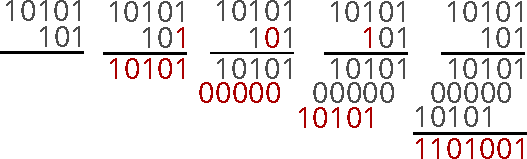
\includegraphics[width=0.5\textwidth]{binary_multiplication}
    \caption{Ukázka postupu násobení 0b010101 $\cdot{}$ 0b0101}\label{fig:binary_multiplication}
\end{figure}

Celočíselné dělení (\verb|mpt_div|) řešíme následovně:
\begin{enumerate}
    \item Najdeme v dělenci část (s nejvyšší vahou), od které lze odečíst dělitel
    \item Ve výsledné hodnotě nastavíme bit na pozici odpovídající LSB nalezené části na jedničku. Od nalezené části dělitel odečteme, a se vzniklým rozdílem pokračujeme
    \item Pokud jsme na konci dělence, algoritmus končí a výslednou hodnotu vrátíme
    \item K rozdílu přidáváme další bity dokud opět nemůžeme odečíst dělitel, poté se vrátíme ke kroku 2 
\end{enumerate}

Tento postup neprovádíme přímo se zadanými operandy, ale s jejich absolutními hodnotami, a pokud má být výsledná hodnota záporná, vrátíme na konci číslo opačné.

Postup dělení je ilustrován na obrázku~\ref{fig:binary_division}.

\begin{figure}[ht]
    \centering
    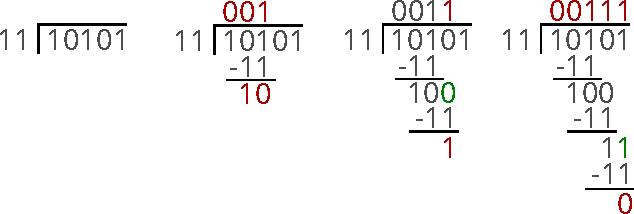
\includegraphics[width=0.5\textwidth]{binary_division}
    \caption{Ukázka postupu dělení 0b010101\textdiv0b011}\label{fig:binary_division}
\end{figure}

Mocnění základu exponentem má v binární soustavě elegantní řešení~\cite{bib:power} popsané pseudokódem~\ref{alg:power}.

\begin{algorithm}[H]
\floatname{algorithm}{Algoritmus}
\caption{Umocnění základu exponentem v binární soustavě}\label{alg:power}
\begin{algorithmic}[1]
\scriptsize{
\Function{Power}{$base, exponent$}
	\If{$exponent = 0$}
		\State{\Return{$0$}}
	\EndIf{}
    \If{$exponent = 1$}
		\State{\Return{$base$}}
	\EndIf{}
    \State{$x:=base$}
    \For{$1$..bit\_count($exponent$)}
        \State{$x:=x^2$}
        \If{get\_bit($exponent$, bit\_count($exponent$)$ - i$)$ = 1$}
            \State{$x = x\cdot base$}
        \EndIf{}
    \EndFor{}
	\State{\Return{$x$}}
\EndFunction{}
}
\end{algorithmic}
\end{algorithm}
\newpage

\subsection{Převod řetězce na MPT}
Funkce pro převody řetězců na \verb|mpt| se nachází v souborech \\ \verb|multiple_precision_parsing.c/.h|.

Pro převod používáme hlavně funkci \verb|mpt_parse_str|, která dokáže rozpoznat v jaké soustavě bylo číslo zadáné podle prefixu (\verb|0b / 0x|) nebo jeho absence. Funkce převádí číslo dokud jsou znaky pro danou soustavu platné a ve chvíli, kdy narazí na znak, který není součástí dané soustavy, ukončí činnost a vrátí hodnotu, kterou se podařilo převést. Během procházení znaků také mění ukazatel zadaný v parametru a na konci převodu bude ukazatel ukazovat na poslední znak, který číslu náležel.

Převod z čísel zadaných v binární soustavě probíhá následovně:
\begin{enumerate}
    \item Vytvoříme instanci \verb|mpt| s názvem \verb|new| a hodnotou 0
    \item Přečteme znak, a pokud nepatří do binární soustavy, ukončíme převod, jinak pokračujeme
    \item Hodnotu \verb|new| bitově posuneme o jednu pozici vlevo
    \item Nastavíme nultý bit \verb|new| na 1 nebo 0 podle aktuálního znaku
    \item Změníme ukazatel na další znak a vrátíme se na krok 2
\end{enumerate}
Převod z čísel zadaných v hexadecimální soustavě probíhá analogicky k binární soustavě s tím rozdílem, že bitový posun vlevo provádíme o čtyři pozice a místo nastavování nultého bitu, přičítáme hodnotu hexadecimálního znaku.

U těchto soustav musíme navíc ještě ošetřit, jestli byla čísla zadána v dvojkovém doplňku a mají být záporná. Např.~\verb|0b1101| by takto bylo převedeno na \verb|0b00001101| a je tedy třeba nastavit potřebné bity zleva na jedničku, k čemuž slouží statická funkce \verb|fill_set_bits_|.

Pro převod z dekadické soustavy používáme následující postup:
\begin{enumerate}
    \item Vytvoříme instanci \verb|mpt| s názvem \verb|new| a hodnotou 0
    \item Přečteme znak, a pokud nepatří do dekadické soustavy, ukončíme převod, jinak pokračujeme
    \item Hodnotu \verb|new| vynásobíme deseti
    \item K \verb|new| přičteme hodnotu znaku v dekadické soustavě.
    \item Změníme ukazatel na další znak a vrátíme se na krok 2
\end{enumerate}

\subsection{Výpisy MPT}
Funkce pro výpisy hodnot \verb|mpt| se nachází v souborech \\ \verb|multiple_precision_printing.c/.h|.

Pro výpis používáme funkci \verb|mpt_print|, která hodnotu vypíše v požadované soustavě.
\\\\
Výpis v binární soustavě je nejjednodušší:
\begin{enumerate}
    \item Vypíšeme '0b' a hodnotu MSB
    \item Ignorujeme všechny bity před (s nižší vahou) MSB, které mají stejnou hodnotu jako MSB
    \item Zbytek bitů vypíšeme v pořadí od nejvyššího po nultý
\end{enumerate} 

Výpis v hexadecimální soustavě provádíme po nibblech (čtveřice bitů) od nejvyššího nibblu po nultý.
\begin{enumerate}
    \item Vypíšeme '0x'
    \item Ignorujeme všechny nibbly s hodnotu \verb|0xf| (když MSB $ = 1$) nebo \verb|0x0| (když MSB $ = 0$)
    \item Pokud MSB $ = 0$ a aktuální nibble $\geq 8$, vypíšeme '0', jinak další krok
    \item Pokud MSB $ = 1$ a aktuální nibble $<8$, vypíšeme '0', jinak další krok
    \item Zbytek nibblů vypíšeme v pořadí od nejvyššího po nultý
\end{enumerate}

Pro výpis v dekadické soustavě si nejprve vytvoříme absolutní hodnotu zadané instance \verb|mpt|. Tu postupně dělíme deseti, kde zbytek po dělení nám postupně dá jednotlivé číslice v dekadické podobě. Číslice takto ale získáváme pozpátku, proto je nejprve ukládáme do vektoru, jehož obsah nakonec pozpátku vypíšeme, ještě před vypsáním vektoru ale vypíšeme znak mínusu, pokud bylo původní číslo záporné.

\subsection{Operátory}
Podporované operátory a k nim přidružené obslužné funkce, precedence a asociativity jsou ve struktuře \verb|func_oper_type| v souborech \verb|operators.c/.h|, spolu s funkcí \verb|get_func_operator| pro získání struktury \verb|func_oper_type| s daty, odpovídajícími požadovanému znaku operátoru.

\subsection{Shunting yard}
Funkce pro zpracování zadaných výrazů se nachází v souborech \verb|shunting_yard.c/.h|.

Shunting yard je implementován standardně podle článku~\cite{bib:shunting_yard} a jeho činnost voláme funkcí \verb|shunt| s tím, že po úspěšném provedení algoritmu nejsou čísla ve výsledné RPN formě zapsána přímo, ale jsou reprezentována znakem 'n' a jejich skutečné \verb|mpt| hodnoty jsou uloženy ve výsledném zásobníku \verb|values|. Při vyhodnocování RPN pak při každém přečtení znaku 'n' skutečnou hodnotu čísla z tohoto zásobníku odebereme. 

Existuje speciální případ infixové formy, kde se, i přes správnou precedenci a asociativitu (podle tab.~\ref{tab:function}), RPN forma vytvoří v nesprávném tvaru, a to umocnění základu zápornou hodnotou např.~ve tvaru '\verb|4^-2|'. Správná forma RPN by byla '\verb|42-^|', s naším algoritmem by ale výsledná RPN forma byla '\verb|4^2-|', která by při vyhodnocování výsledku vrátila chybu. Z toho důvodu je tento speciální případ ošetřen ve statické funkci \verb|shunt_minus_| tak, že se operátor mínusu vynechá, zpracuje se výraz za mínusem a mínus se přidá do výsledné RPN formy naposled.

\begin{figure}[ht]
    \centering 
    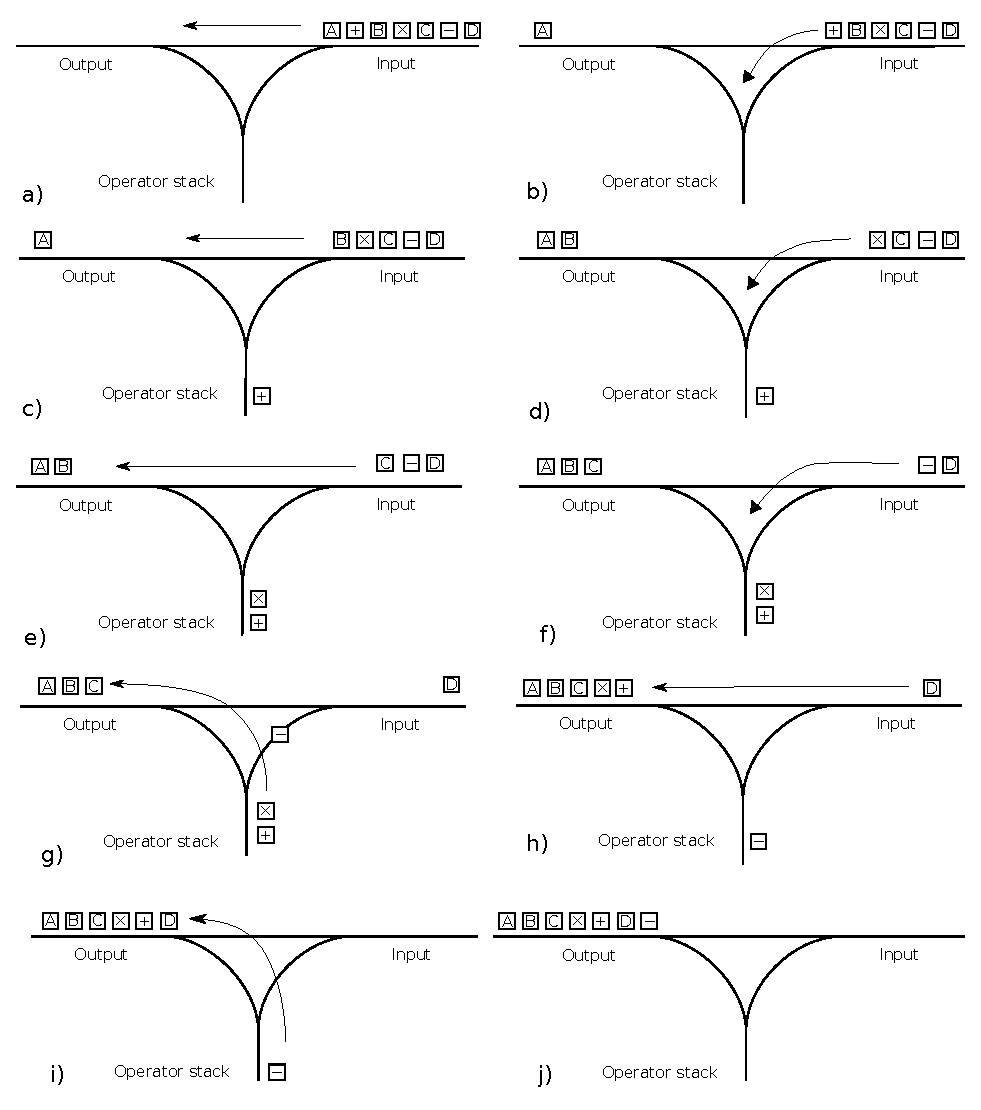
\includegraphics[width=0.8\textwidth]{shunting_yard}
    \caption{Ilustrace postupu algoritmu Shunting yard (převzato z~\cite{bib:shunting_yard}).}\label{fig:shunting_yard}
\end{figure}

\subsection{Vyhodnocení RPN}
Funkce pro vyhodnocení RPN se nachází v souborech \verb|shunting_yard.c/.h|.

Vyhodnocení výrazů ve formě RPN je také implementováno standardně. V algoritmu se využívá zásobník \verb|stack_values| pro mezivýsledky. Znaky výrazu zpracováváme jeden po druhém. Pokud narazíme na znak 'n', do \verb|stack_values| vložíme hodnotu \verb|mpt| odebranou ze zásobníku \verb|values|. Pokud je znak operátor, provedeme odpovídající operaci nad hodnotou, resp.~hodnotami odstraněnými ze zásobníku \verb|stack_values| a výsledek do stejného zásobníku vložíme.

Na konci vyhodnocení by se v zásobníku \verb|stack_values| měla nacházet jediná (výsledná) hodnota, a pokud tomu tak není, obsahoval výraz syntaktickou chybu.

\section{Uživatelská příručka}
\subsection{Přeložení a sestavení programu}
Postup pro přeložení a sestavení je na všech platformách stejný. Je nutné mít nainstalovaný překladač \verb|gcc| a nástroj \verb|make| a mít zprovozněné jejich ekvivalentní příkazy v konzoli. Samotný překlad a sestavení provedeme v příkazovém řádku v kořenové složce programu příkazem \verb|make|. Po úspěšném sestavení se ve stejném adresáři vytvoří spustitelný binární soubor \verb|calc.exe|.

\begin{figure}[ht]
    \centering
    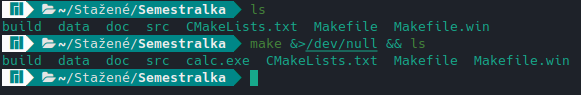
\includegraphics[width=0.8\textwidth]{sestaveni.png}
    \caption{Ukázka překladu a sestavení programu}\label{fig:sestaveni}
\end{figure}

\subsection{Spuštění a ovládání programu}
Program spouštíme, podle zadání, dvěma způsoby. 

Příkazem \verb|calc.exe| program otevřeme v interaktivním režimu (viz obr.~\ref{fig:ukazka_interaktivni}) pro postupné zadávání příkazů nebo infixových výrazů z příkazové řádky. Zadáním nepodporovaného příkazu nebo výrazu se špatnou syntaxí vypíše program odpovídající chybovou hlášku a čeká na nový příkaz. Příkazem \verb|quit| program ukončíme.

Příkazem \verb|calc.exe [<vstupni-soubor>]| program načte vstupní soubor, každý řádek v něm zpracuje jako zadaný výraz, řádek vypíše jako bychom ho zadali v interaktivním režímu a následně vypíše výsledek zpracování (viz obr.~\ref{fig:ukazka_soubor}). Po zpracování všech řádků v souboru se program ukončí s návratovou hodnotou \verb|EXIT_SUCCESS|. Pokud zadaný soubor neexistuje vypíše chybovou hlášku a skončí s návratovou hodnotou \verb|EXIT_FAILURE|. 
\newpage
\begin{figure}[ht]
    \centering
    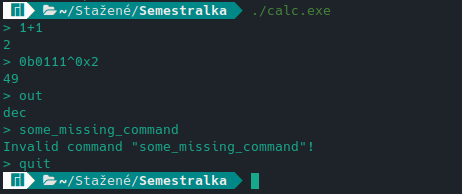
\includegraphics[width=0.8\textwidth]{ukazka_interaktivni.png}
    \caption{Ukázka interaktivního režimu}\label{fig:ukazka_interaktivni}
\end{figure}
\begin{figure}[ht]
    \centering
    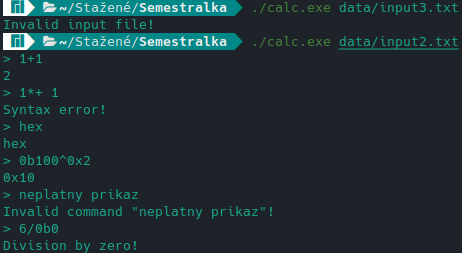
\includegraphics[width=0.8\textwidth]{ukazka_soubor.png}
    \caption{Ukázka načtení a zpracování souboru}\label{fig:ukazka_soubor}
\end{figure}
\newpage
\section{Závěr}
Vytvořená kalkulačka dokáže provádět všechny požadované operace, často i za relativně krátkou dobu běhu. Výrazy v infixové formě zpracovat umí a během testovaní nebyl nalezen žádný výraz, který by se vyhodnotil nesprávně. Speciální případ výrazu s operátorem mocniny, po kterém následuje operátor negace, je ošetřen, správnost tohoto ošetření nemusí být ale jednoznačná pro některé složitější výrazy. Implementovány jsou jak režim interaktivní, tak režim zpracování souboru, včetně chybových hlášení nepodporovaných příkazů, či nedefinovaných matematických operací. `Nekonečně velká' čísla sice kalkulačka zpracovat neumí, čísla ale mohou být tak velká, že je lze označit za `prakticky nekonečně velká'.

Jedním z problému k vyřešení byla příliš dlouhá doba kontroly programem \verb|valgrind|, která byla  způsobena zbytečnými dynamickými alokacemi a realokacemi struktury \verb|mpt| a bylo nutné celý program přepsat tak, aby se struktury alokovaly na zásobníku. 
Rychlost vyhodnocování některých výrazů může u větších čísel být relativně malá a určitě existují algoritmy, které by byly pro provedení vybraných matematických operací lepší. Právě takové algoritmy pravděpodobně využívá např.~knihovna \href{https://gmplib.org/}{\textit{GMP}}, která je lepší alternativou našeho řešení.

\begin{thebibliography}{1}
\bibitem{bib:zadani}
\small{Úplné zadání
[Online]\\
\url{https://www.kiv.zcu.cz/studies/predmety/pc/data/works/sw2022-03.pdf}
}
\bibitem{bib:bit_array}
\small{Bitové pole
[Online]\\
\url{https://en.wikipedia.org/wiki/Bit_array}
}
\bibitem{bib:adder}
\small{Binární sčítačka
[Online]\\
\url{https://cs.wikipedia.org/wiki/Bin%C3%A1rn%C3%AD_s%C4%8D%C3%ADta%C4%8Dka}
}
\bibitem{bib:power}
\small{Algoritmus binárního umocňování
[Online]\\
\url{https://cs.wikipedia.org/wiki/Algoritmus_bin%C3%A1rn%C3%ADho_umoc%C5%88ov%C3%A1n%C3%AD}
}
\bibitem{bib:rpn}
\small{Reverzní Polská notace
[Online]\\
\url{https://en.wikipedia.org/wiki/Reverse_Polish_notation}
}
\bibitem{bib:shunting_yard}
\small{Algoritmus Shunting yard
[Online]\\
\url{https://en.wikipedia.org/wiki/Shunting_yard_algorithm}
}
\end{thebibliography}
\addcontentsline{toc}{section}{Odkazy}

\end{document}